% В этом файле следует писать текст работы, разбивая его на
% разделы (section), подразделы (subsection) и, если нужно,
% главы (chapter).

% Предварительно следует указать необходимую информацию
% в файле SETUP.tex

%% В этот файл не предполагается вносить изменения

% В этом файле следует указать информацию о себе
% и выполняемой работе.

\documentclass [fontsize=14pt, paper=a4, pagesize, DIV=calc]%
{scrreprt}
% ВНИМАНИЕ! Для использования глав поменять
% scrartcl на scrreprt

% Здесь ничего не менять
\usepackage [T2A] {fontenc}   % Кириллица в PDF файле
\usepackage [utf8] {inputenc} % Кодировка текста: utf-8
\usepackage [russian] {babel} % Переносы, лигатуры

%%%%%%%%%%%%%%%%%%%%%%%%%%%%%%%%%%%%%%%%%%%%%%%%%%%%%%%%%%%%%%%%%%%%%%%%
% Создание макроса управления элементами, специфичными
% для вида работы (курс., бак., маг.)
% Здесь ничего не менять:
\usepackage{ifthen}
\newcounter{worktype}
\newcommand{\typeOfWork}[1]
{
	\setcounter{worktype}{#1}
}

% ВНИМАНИЕ!
% Укажите тип работы: 0 - курсовая, 1 - бак., 2 - маг.,
% 3 - бакалаврская с главами.
\typeOfWork{3}
% Считается, что курсовая и бак. бьются на разделы (section) и
% подразделы (subsection), а маг. — на главы (chapter), разделы и
%  подразделы. Если хочется,
% чтобы бак. была с главами (например, если она большая),
% надо выбрать опцию 3.

% Если при выборе 2 или 3 вы забудете поменять класс
% документа на scrreprt (см. выше, в самом начале),
% то получите ошибку:
% ./aux/appearance.tex:52: Package scrbase Error: unknown option ` chapterprefix=

%%%%%%%%%%%%%%%%%%%%%%%%%%%%%%%%%%%%%%%%%%%%%%%%%%%%%%%%%%%%%%%%%%%%%%%%
% Информация об авторе и работе для титульной страницы

\usepackage {titling}

% Имя автора в именительном падеже (для маг.)
%%\newcommand {\me}{%
%%И.\,И.~Иванов
%%}

% Имя автора в родительном падеже (для курсовой и бак.)
\newcommand {\byme}{%
A.\,A.~Мухаррам
}

% Любимый научный руководитель
\newcommand{\supervisor}%
{ст. преп. В. Н. Брагилевский}

% идентифицируем пол (только для курсовой и бак.)
\newcommand{\bystudent}{
студентки %студентки % Для курсовой: с большой буквы
}

% Год публикации
\date{2015}

% Название работы
\title{Реализация интервального времени в RabbitMQ}

% Кафедра
%
\newboolean{needchair}
\setboolean{needchair}{true} % на ФИИТ не пишется (false), на ПМИ есть (true)

\newcommand {\thechair} {%
Кафедра информатики и вычислительного эксперимента%
}

\newcommand {\direction} {%
Направление подготовки\\
Прикладная математика и информатика%
}% 

%%%%%%%%%%%%%%%%%%%%%%%%%%%%%%%%%%%%%%%%%%%%%%%%%%%%%%%%%%%%%%%%%%%%%%%%
% Другие настраиваемые элементы текста

% Листинги с исходным кодом программ: укажите язык программирования
\usepackage{listings}
\lstset{
    language=erlang,%  Язык указать здесь
    basicstyle=\small\ttfamily,
    breaklines=true,%
    showstringspaces=false%
    inputencoding=utf8x%
}
% полный список языков, поддерживаемых данным пакетом, есть,
% например, здесь (стр. 13):
% ftp://ftp.tex.ac.uk/tex-archive/macros/latex/contrib/listings/listings.pdf

% Гиперссылки: настройте внешний вид ссылок
\usepackage%
[pdftex,unicode,pdfborder=0,draft=false,%backref=page,
    hidelinks, % убрать, если хочется видеть ссылки: это
               % удобно в PDF файле, но не должно появиться на печати
    bookmarks=true,bookmarksnumbered=false,bookmarksopen=false]%
{hyperref}


\usepackage {amsmath}      % Больше математики
\usepackage {amssymb}
\usepackage {textcase}     % Преобразование к верхнему регистру
\usepackage {indentfirst}  % Красная строка первого абзаца в разделе

\usepackage {fancyvrb}     % Листинги: определяем своё окружение Verb
\DefineVerbatimEnvironment% с уменьшенным шрифтом
	{Verb}{Verbatim}
	{fontsize=\small}

% Вставка рисунков
\usepackage {graphicx}

% Общее оформление
% ----------------------------------------------------------------
% Настройка внешнего вида

%%% Шрифты

% если закомментировать всё — консервативная гарнитура Computer Modern
\usepackage{paratype} % профессиональные свободные шрифты
%\usepackage {droid}  % неплохие свободные шрифты от Google
%\usepackage{mathptmx}
%\usepackage {mmasym}
%\usepackage {psfonts}
%\usepackage{lmodern}
%var1: lh additions for bold concrete fonts
%\usepackage{lh-t2axccr}
%var2: the package below could be covered with fd-files
%\usepackage{lh-t2accr}
%\usepackage {pscyr}

% Геометрия текста

\usepackage{setspace}       % Межстрочный интервал
\onehalfspacing

\newlength\MyIndent
\setlength\MyIndent{1.25cm}
\setlength{\parindent}{\MyIndent} % Абзацный отступ
\frenchspacing            % Отключение лишних отступов после точек
\KOMAoptions{%
    DIV=calc,         % Пересчёт геометрии
    numbers=endperiod % точки после номеров разделов
}

                            % Консервативный вариант:
%\usepackage                % ручное задание геометрии
%[%                         % (не рекомендуется в проф. типографии)
%  margin = 2.5cm,
  %includefoot,
  %footskip = 1cm
%] %
%  {geometry}

%%% Заголовки



\ifthenelse{\equal{\theworktype}{2}}{%
\KOMAoptions{%
    numbers=endperiod,% точки после номеров разделов
    headings=normal,   % размеры заголовков поменьше стандартных
    chapterprefix=true,% Печатать слово Глава в магистерской
    appendixprefix=true% Печатать слово Приложение
}
}

% шрифт для оформления глав и названия содержания
\newcommand{\SuperFont}{\Large\sffamily\bfseries}

% Заголовок главы
\ifthenelse{\value{worktype} > 1}{%
\renewcommand{\SuperFont}{\Large\normalfont\sffamily}
\newcommand{\CentSuperFont}{\centering\SuperFont}
\usepackage{fncychap}
\ChNameVar{\SuperFont}
\ChNumVar{\CentSuperFont}
\ChTitleVar{\CentSuperFont}
\ChNameUpperCase
\ChTitleUpperCase
}

% Заголовок (под)раздела с абзацного отступа
\addtokomafont{sectioning}{\hspace{\MyIndent}}

\renewcommand*{\captionformat}{~---~}
\renewcommand*{\figureformat}{Рисунок~\thefigure}

%%% Оглавление
\usepackage{tocloft}

% шрифт и положение заголовка
\ifthenelse{\value{worktype} > 1}{%
\renewcommand{\cfttoctitlefont}{\hfil\SuperFont\MakeUppercase}
}{
\renewcommand{\cfttoctitlefont}{\hfil\SuperFont}
}

% слово Глава
\usepackage{calc}
\ifthenelse{\value{worktype} > 1}{%
\renewcommand{\cftchappresnum}{Глава }
\addtolength{\cftchapnumwidth}{\widthof{Глава }}
}

% Очищаем оформление названий старших элементов в оглавлении
\ifthenelse{\value{worktype} > 1}{%
\renewcommand{\cftchapfont}{}
\renewcommand{\cftchappagefont}{}
}{
\renewcommand{\cftsecfont}{}
\renewcommand{\cftsecpagefont}{}
}

\ifthenelse{\value{worktype} > 1}{%
    \renewcommand{\cftchapaftersnum}{.}
}{
\renewcommand{\cftsecaftersnum}{.}
\renewcommand{\cftsubsecaftersnum}{.}
}
%%% Списки (enumitem)

\usepackage {enumitem}      % Списки с настройкой отступов
\setlist %
{ %
  leftmargin = \parindent, itemsep=.5ex, topsep=.4ex
} %

% По ГОСТу нумерация должны быть буквами: а, б...
%\makeatletter
%    \AddEnumerateCounter{\asbuk}{\@asbuk}{м)}
%\makeatother
%\renewcommand{\labelenumi}{\asbuk{enumi})}
%\renewcommand{\labelenumii}{\arabic{enumii})}

%%% Таблицы: выбрать более подходящие

\usepackage{booktabs} % считаются наиболее профессионально выполненными
%\usepackage{ltablex}
%\newcolumntype {L} {>{---}l}

%%% Библиография

\usepackage{csquotes}        % Оформление списка литературы
\usepackage[
  backend=biber,
  hyperref=auto,
  language=auto,
  citestyle=gost-numeric,
  bibstyle=gost-numeric,
]{biblatex}
\addbibresource{biblio.bib} % Файл с лит.источниками

% Настройка величины отступа в списке
\ifthenelse{\value{worktype} < 2}{%
\defbibenvironment{bibliography}
  {\list
     {\printtext[labelnumberwidth]{%
    \printfield{prefixnumber}%
    \printfield{labelnumber}}}
     {\setlength{\labelwidth}{\labelnumberwidth}%
      \setlength{\leftmargin}{\labelwidth}%
      \setlength{\labelsep}{\dimexpr\MyIndent-\labelwidth\relax}% <----- default is \biblabelsep
      \addtolength{\leftmargin}{\labelsep}%
      \setlength{\itemsep}{\bibitemsep}%
      \setlength{\parsep}{\bibparsep}}%
      \renewcommand*{\makelabel}[1]{\hss##1}}
  {\endlist}
  {\item}
}{}

% ----------------------------------------------------------------
% Настройка переносов и разрывов страниц

\binoppenalty = 10000      % Запрет переносов строк в формулах
\relpenalty = 10000        %

\sloppy                    % Не выходить за границы бокса
%\tolerance = 400          % или более точно
\clubpenalty = 10000       % Запрет разрывов страниц после первой
\widowpenalty = 10000      % и перед предпоследней строкой абзаца

% ----------------------------


% Стили для окружений типа Определение, Теорема...
% Оформление теорем (ntheorem)

\usepackage [thmmarks, amsmath] {ntheorem}
\theorempreskipamount 0.6cm

\theoremstyle {plain} %
\theoremheaderfont {\normalfont \bfseries} %
\theorembodyfont {\slshape} %
\theoremsymbol {\ensuremath {_\Box}} %
\theoremseparator {:} %
\newtheorem {mystatement} {Утверждение} [section] %
\newtheorem {mylemma} {Лемма} [section] %
\newtheorem {mycorollary} {Следствие} [section] %

\theoremstyle {nonumberplain} %
\theoremseparator {.} %
\theoremsymbol {\ensuremath {_\diamondsuit}} %
\newtheorem {mydefinition} {Определение} %

\theoremstyle {plain} %
\theoremheaderfont {\normalfont \bfseries} 
\theorembodyfont {\normalfont} 
%\theoremsymbol {\ensuremath {_\Box}} %
\theoremseparator {.} %
\newtheorem {mytask} {Задача} [section]%
\renewcommand{\themytask}{\arabic{mytask}}

\theoremheaderfont {\scshape} %
\theorembodyfont {\upshape} %
\theoremstyle {nonumberplain} %
\theoremseparator {} %
\theoremsymbol {\rule {1ex} {1ex}} %
\newtheorem {myproof} {Доказательство} %

\theorembodyfont {\upshape} %
%\theoremindent 0.5cm
\theoremstyle {nonumberbreak} \theoremseparator {\\} %
\theoremsymbol {\ensuremath {\ast}} %
\newtheorem {myexample} {Пример} %
\newtheorem {myexamples} {Примеры} %

\theoremheaderfont {\itshape} %
\theorembodyfont {\upshape} %
\theoremstyle {nonumberplain} %
\theoremseparator {:} %
\theoremsymbol {\ensuremath {_\triangle}} %
\newtheorem {myremark} {Замечание} %
\theoremstyle {nonumberbreak} %
\newtheorem {myremarks} {Замечания} %


% Титульный лист
% Макросы настройки титульной страницы
% В этот файл не предполагается вносить изменения

%\usepackage {showframe}

% Вертикальные отступы на титульной странице
\newcommand{\vgap}{\vspace{10pt}}

% Помещение города и даты в нижний колонтитул
\usepackage{scrlayer}
\DeclareNewLayer[
  foot,
  foreground,
  contents={%
    \raisebox{\dp\strutbox}[\layerheight][0pt]{%
      \parbox[b]{\layerwidth}{\centering Ростов-на-Дону\\ \thedate%
       \\\mbox{}
       }}%
  }
]{titlepage.foot.fg}
\DeclareNewPageStyleByLayers{titlepage}{titlepage.foot.fg}


\AtBeginDocument %
{ %
  %
  \begin{titlepage}
  %
    \thispagestyle{titlepage}

    {\centering
    %
    \MakeTextUppercase {МИНИСТЕРСТВО ОБРАЗОВАНИЯ И НАУКИ РФ}

    \vgap

    Федеральное государственное автономное образовательное\\
    учреждение высшего образования\\
    \MakeTextUppercase {Южный федеральный университет}

    \vgap

  Институт математики, механики и компьютерных наук
    им.~И.\,И.~Воровича

    \vgap

    \direction

    \ifthenelse{\boolean{needchair}}{
    \vgap

    \thechair}{}

    \vspace* {\fill}

    \ifthenelse{\value{worktype} = 2}{%
    \me

    \vgap}{}

    \MakeTextUppercase{\thetitle}

    \ifthenelse{\value{worktype} = 2}{%
     \vgap

    Магистерская диссертация}{}
    \ifthenelse{\value{worktype} = 0}{
     \vgap

    Курсовая работа
    }{}%

    \vspace {\fill}

    \begin{flushright}
    \ifthenelse{\value{worktype} = 1 \OR \value{worktype} = 3}{
    Выпускная квалификационная работа\\
    на степень бакалавра%
   }{}%
    \ifthenelse{\value{worktype} = 1 \OR \value{worktype} = 0 \OR \value{worktype} = 3}{%
    \bystudent\\
    \byme
    }{}

    \vgap

    Научный руководитель:\\
    \supervisor\\
    \ifthenelse{\value{worktype} = 2}{%
    Рецензент:\\
    ученая степень, ученое звание [, должность]
    И. О. Фамилия
    }{}
  \end{flushright}

    \vspace {\fill}

  %Ростов-на-Дону

    %\thedate

  }\end{titlepage}
  %
  %
  \tableofcontents
  %
  \clearpage
} %



% Команды для использования в тексте работы


% макросы для начала введения и заключения
\newcommand{\Intro}{\addsec{Введение}}
\ifthenelse{\value{worktype} > 1}{%
    \renewcommand{\Intro}{\addchap{Введение}}%
}

\newcommand{\Conc}{\addsec{Заключение}}
\ifthenelse{\value{worktype} > 1}{%
    \renewcommand{\Conc}{\addchap{Заключение}}%
}

% Правильные значки для нестрогих неравенств и пустого множества
\renewcommand {\le} {\leqslant}
\renewcommand {\ge} {\geqslant}
\renewcommand {\emptyset} {\varnothing}

% N ажурное: натуральные числа
\newcommand {\N} {\ensuremath{\mathbb N}}

% значок С++ — используйте команду \cpp
\newcommand{\cpp}{C\nolinebreak\hspace{-.05em}%
\raisebox{.2ex}{+}\nolinebreak\hspace{-.10em}%
\raisebox{.2ex}{+}}

% Неразрывный дефис, который допускает перенос внутри слов,
% типа жёлто-синий: нужно писать жёлто"/синий.
\makeatletter
    \defineshorthand[russian]{"/}{\mbox{-}\bbl@allowhyphens}
\makeatother


\endinput

% Конец файла


\begin{document}

\Intro

Отсутствие глобального соглашения о времени может привести к возникновению ошибок в системе. В таких случаях принято говорить о необходимости синхронизации часов.
Синхронизация часов связана с пониманием порядка следования во времени событий конкурентных процессов. Она может быть полезна в тех случаях, когда необходимо синхронизировать обмен сообщениями, контролировать совместное использование ресурсов и выполнение совместной работы несколькими процессами. Таким образом, задача синхронизации в распределенной системе - обеспечить возможность принятия согласованного решения процессами о порядке следования событий. \par
Одним из вариантов решения данной проблемы является использование логических часов. Этот механизм впервые был предложен и реализован Лэсли Лампортом в 1978 году.
В своей статье [1] он указал, что обычно имеет значение не точное время выполнения события процесса, а его порядок. \par
Лампорт определил логические часы как способ присвоить номер событию, где под номером понимается время, в которое наступило событие. Для каждого процесса $P_i$ определяются часы $C_i$ как функция, которая ставит в соответствие каждому событию $a$ процесса $P_i$ число  $C_i(a)$. Система в целом описывается с помощью функции $C$, которая ставит в соответствие каждому событию $b$ число $C(b)$, 
где $C(b)=$ $C_j(b)$, если $b$ - событие процесса $P_j$. С помощью этой функции можно сравнивать время наступления событий в распределенной системе.\par
Интервальные отметки времени - один из алгоритмов логических часов.  
В данной работе описан процесс разработки плагина для брокера сообщений RabbitMQ, реализующего мониторинг событий брокера на основе интервальных отметок времени. С помощью данного плагина можно восстановить цепочку событий между любыми двумя событиями системы. Под событием в RabbitMQ будет подразумеваться отправка или получение сообщения. 
\newpage

% Если typeOfWork в SETUP.tex задан как 2 или 3, то начинать
% надо не с section (раздел), а с главы (chapter)
\chapter{Логические часы}
\label{sec:examples}
Эта глава будет посвящена рассмотрению синхронизации процессов посредством нескольких алгоритмов логических часов.\par
Введем основные понятия. 
Для синхронизации логических часов Лампорт определил  не рефлексивное, транзитивное отношение под названием \textquote{происходит раньше}, которое удовлетворяет следующим 3 условиям: 
\begin{itemize}
\item Если $a$ и $b$ — события, происходящие в одном и том же процессе, и $a$
           происходит раньше, чем $b$, то отношение $a \rightarrow b$ истинно.
\item Если $a$ - отправка сообщения одним процессом, а $b$ - это получения этого сообщения другим процессом, то отношение $a \rightarrow b$ истинно.
\item Если $a \rightarrow c$ и $c \rightarrow b$, тогда из $a \rightarrow b$
\end{itemize}
Два отдельных события $a$ и $b$ конкурентные, если оба отношения $a \rightarrow b$ и $b \rightarrow a$ несправедливы. \par
Основываясь на введенном отношении и функции логических часов, запишем условие:
для любых двух событий $a$ и $b$, если $a \rightarrow b$ истинно, то $C(a) < C(b)$. Ясно, что это условие выполняется, если  события $a$ и $b$ удовлетворяют одному из условий перечисленных выше. \par
Рассмотрим последовательность событий, происходящих между тремя процессами, изображенную на рисунке 1.1.
\begin{figure}
\centering

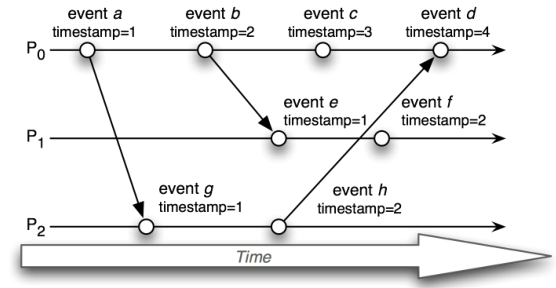
\includegraphics[width=0.5\textwidth]{img/lamport1.png}
\caption{неупорядоченная последовательность событий}
\end{figure}
Процессы запущены на разных машинах, каждая из которых имеет собственные часы и скорость работы. Каждый процесс поддерживает свой глобальный счетчик, который увеличивается на единицу перед тем, как присвоить новому событию временную отметку. Анализируя временные отметки событий, изображенных на рисунке 1.1, можно заметить несколько особенностей. Событие $g$, событие изображающее получение сообщения, посланного событием $a$, имеет такую же временную отметку, что и событие $a$, хотя совершенно ясно, что оно произошло после события $a$. Событие $e$ имеет  временную отметку меньше, чем событие отправившее ему сообщение (событие $b$).

\section{Временные отметки Лампорта}
Алгоритм Лампорта исправляет ситуацию, описанную выше, перенумеровывая временные отметки так, чтобы для событий, относящихся к отправке и получению сообщений, выполнялось отношение \textquote{происходит раньше}. \par
Правила:
\begin{itemize}
\item Каждый процесс имеет счетчик, который увеличивается на единицу  перед каждым внутренним событием процесса. Событиями процесса считается получение и отправка сообщений. 
\item К сообщению при отправке прикрепляется значение счетчика процесса.
\item При получении сообщения, если значение счетчика процесса-получателя меньше временной отметки полученного сообщения, процесс-получатель меняет значение счетчика на значение полученной временной отметки, иначе ничего не меняется. 
\end{itemize}
Применив этот алгоритм к последовательности сообщений, изображенной на рисунке 1.1, мы получим правильно упорядоченный поток сообщений среди событий, связанных 
причинно-следственной связью (рисунок 1.2). 
\begin{figure}
\centering
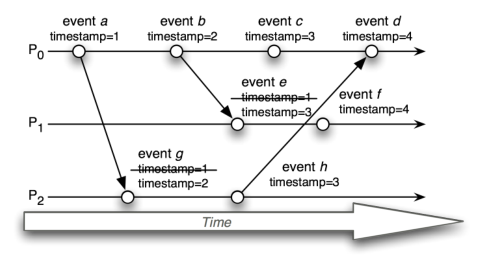
\includegraphics[width=0.5\textwidth]{img/lamport2.png}
\caption{упорядоченная последовательность событий}
\end{figure}
Каждое событие системы теперь имеет временную отметку, которая называется временной отметкой Лампорта. В условиях выполнения правил данного алгоритма, для любых двух событий системы $a$ и $b$ , если отношение $a \rightarrow b$ истинно, то $L(a) < L(b)$, где $L(x)$ - временная отметка Лампорта для события $x$. 

\section{Векторные отметки времени} 
Благодаря алгоритму Лампорта события в системе имеют единую последовательность, однако из сравнения временных отметок Лампорта $L(a)$ и $L(b)$  нельзя сделать вывод о взаимосвязи между событиями $a$ и $b$. Причинно-следственная связь может быть установлена посредством векторных
отметок времени (vector timestams).Этот алгоритм был независимо предложен Маттерном в 1989 г.(Mattern) и Фиджем в 1991 г. (Fidge).\par
Векторная отметка времени в системе из $N$ процессов - целочисленный вектор длины $N$.\par
Правила для использования векторных отметок времени:  
\begin{itemize}
\item Каждый процесс в системе имеет свою локальную копию вектора (вектор $V_i$ для процесса $P_i$), которая инициализируется $0$: $V_i[j] = 0, i,j = 1..N$ 
\item Процесс $P_j$ перед каждым новым внутреннем событием увеличивает свою компоненту вектора на единицу: $V_j[j] = V_j[j] + 1$
\item Сообщение отправляется процессом $P_i$ вместе с векторной отметкой времени $V_i$
\item При получении сообщения процесс $P_j$ сравнивает полученную временную отметку $t$ со своим локальным вектором поэлементно, устанавливая каждую компоненту локальной временной отметки как максимум из двух значений: $V_j[i] = max(V_j[i],t[i]), i = \overline{1,N}$
\end{itemize}
Сравниваются векторные отметки по определению: 
\begin{center}
$V = V'$, если $V[i] = V'[i]$, $i = \overline{1,N}$ \\
$V \leq V'$, если $V[i] \leq V'[i]$, $i = \overline{1,N}$ 
\end{center}
С помощью алгоритма векторных часов получаем следующие утверждения:
\begin{center}
Если отношение $a \rightarrow b$ истинно, то $V(a) < V(b)$\\
Если $V(a) < V(b)$, то отношение $a \rightarrow b$ истинно \\
Два события $a$ и $b$ называются конкурентными, если высказываение $V(a)\leq V(b)$ or $V(b)\leq V(a)$ ложно
\end{center}
Рассмотрим последовательность событий, изображенную на рисунке 1.3. Можно заметить, что события $a$ и $e$ конкурентные,т.к. не каждый элемент одного вектора меньше или равен соответствующему элементу другого, а события $b$ и $c$ взаимосвязаны. 

\begin{figure}
\centering
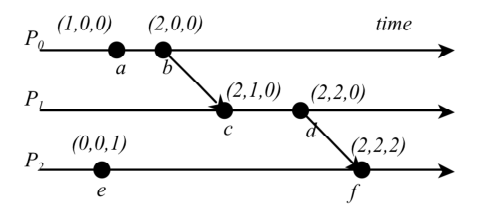
\includegraphics[width=0.5\textwidth]{img/vector.jpg}
\caption{векторный алгоритм}
\end{figure}

\section{Счетчики дерева интервалов: Логические часы для динамических систем}
Хотя отслеживание взаимосвязей между событиями в системах с динамическим изменением числа участников возможно с помощью модифицированного алгоритма векторных часов, в большинстве таких алгоритмов наблюдается чрезмерный структурный рост, а также локализованное удаление не является поддерживаем процессов.  Решение этих проблем возможно с использованием алгоритма счетчиков дерева интервалов (Interval Tree clocks).\par
Данному механизму не требуются глобальные идентификаторы, он способен автономно создавать, удалять и повторно использовать их без помощи глобальной координации; любой объект может создать дочерний объект и количество участников может быть сокращено путем присоединения к произвольным парам объектов; метки могут расти или сокращаться, адаптируясь к динамической природе системы.\par
Механизм отслеживания причинно-следственной связи для алгоритма интервального времени моделируется посредством ряда основных операций: порождения нового процесса($fork$), события($event$) и слияния($join$), воздействующих на интервальные отметки времени (логические часы), чья структура представляет собой пару (i,e), образованную идентификатором и событием, в котором и содержатся все возможные причинно-следственные связи.\par
Основная идея алгоритма заключается в том, что идентификатор каждого участника является множеством интервалов, которые используются для увеличения компоненты событие при наступлении внутреннего события процесса и для передачи последующим элементам при порождении нового процесса.\par 
Рассмотрим операции над интервальными отметками времени.\\
При выполнении операция $\textbf{fork}$ сохраняется компонента событие, а идентификатор делится на два непересекающихся интервала: $fork(i,e) = ((i_1,e),(i_2,e))$  
Операция $peek$ - частный случай операции $fork$: $peek(i,e)=((0,e),(i,e))$\\
Операция $\textbf{event}$ добавляет новое событие к временной отметке (не анонимной, $(0,e)$) так, что, если $event(i,e) = (i,e')$, то $e < e'$. 
Обнаружение причинно-следственной связи на основе интервальных отметок осуществляется посредством сравнения компонент событие.\\
Операция $\textbf{join}$ осуществляет слияние двух отметок: $join((i_1,e_1),(i_2,e_2)) = (i_3,e_3)$, где
$e_3 > e_2$, $e_3 > e_1$, $e_3 = e_2 \sqcup e_1$, $i_3 = f(i_2,i_3)$, $i_3$ уникален на уровне системы.
\par
Классические операции отправки, получения и синхронизации реализуются как композиция основных операций:
\begin{center}
$send = peek \circ event$\\
$receive = event \circ join$\\
$sync = fork \circ join$
\end{center}
В ITC используется исходная метка ($seed$), $(1,0)$, из которой можно получить необходимое число участников $N$ с помощью применения к ней операции $fork$ $N$ раз.
Рассмотрим пример, изображенный на рисунке 1.4. В ITC используется графическая нотация, нижний слой отметки времени - изображение идентификатора, верхние - событие. 
\begin{figure}
\centering
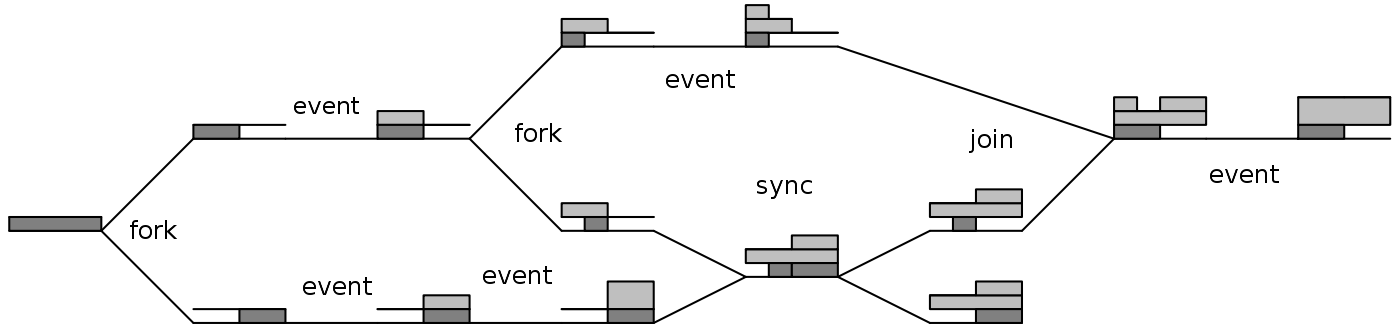
\includegraphics[width=0.8\textwidth]{img/tree.png}
\caption{интервальные отметки времени}
\end{figure}
Работа алгоритма начинается с единственного участника ($seed$) с исходной меткой, которая преобразовывается в две временные отметки под действием операции fork. На данный момент в системе два участника. В поддереве участника, соответсвующего верхней ветке дерева интервалов,происходит внутреннее событие с последующим за ним порождением нового процесса ($fork$). В поддереве участника, соответствующего нижней ветке, происходит два новых события. В этот момент число участников выросло до трех. Затем один из участников подвергается действию события, в то время как оставшиеся два участника синхронизируются. В результате с помощью операции $join$ происходит объединением двух поддеревьев. Этот пример показывает, как просто ITC адаптируется к числу участников системы.


\end{document}
